
Come già accennato in precedenza, l'imponente affermazione mediatica delle blockchain ha contribuito a una crescita significativa dell'attenzione verso lo sviluppo di strumenti e software volti a migliorare l'interpretazione e l'analisi di tali strutture.
Considerata inoltre la quantità di dati presenti in quest'ultime, gli aspetti fondamentali da considerare riguardano il loro immagazzinamento e l'efficienza cui è possibile utilizzarli.

L'utilizzo dei database a grafo rappresenta una grande rivoluzione per la gestione di dati complessi, eterogenei ed interconnessi, i quali, a differenza di quelli relazionali permettono di interrogare relazioni intricate in modo più semplice e naturale, particolarmente utili nel contesto delle blockchain, dove le transazioni e le loro relazioni devono essere tracciate in modo preciso. Inoltre, offrono una soluzione più scalabile migliorando le prestazioni e aprendo nuove possbilità per l'analisi complessa dei dati, la quale necessita di un sistema di reperimento delle informazioni molto efficiente ed efficace.

L'obiettivo principale di questo progetto di tesi è quello di mettere a disposizione ai suddetti strumenti, i dati della blockchain di Bitcoin, tramite lo sviluppo di una base di dati a grafo ed un sistema di API in grado di permetterne un'estrapolazione più efficace ed efficiente.
Nonostante la possibilità di estrarre anche dati generici tramite l'API, il suo sviluppo è incentrato sull'interazione del database con un particolare sistema denominato \textit{BITVAS}.



\subsection{Cenni BITVAS}

BITVAS \cite{TesiBITVAS} è un tool di visualizzazione, sviluppato da Elisa Spigarelli con lo scopo di facilitare le analisi dei dati relativi alla blockchain di Bitcoin.
Il sistema è interattivo e permette agli utenti di selezionare specifiche informazioni tramite un'interfaccia grafica accessibile tramite browser.

Lo sviluppo di un adeguato \emph{paradigma visuale} ha reso più semplice la comprensione della  massiccia mole di dati di cui è composta la struttura dati.
Infatti, a differenza degli altri sistemi, che si concentrano su una visione d'insieme di tutta la struttura, spesso di difficile interpretazione, BITVAS si concentra sulla visualizzazione di un numero minore di dati, permettendo l'analisi di alcuni aspetti altrimenti non valutabili.

Le informazioni trattate riguardano principalmente blocchi, le transazioni e i miner.
L'attenzione è focalizzata sulle relazioni tra blocchi, presenti nella maggior parte delle visualizzazioni sviluppate, in grado di restituire informazioni riguardo i volumi di cryptovaluta scambiati in un derterminato arco temporale.
\newpage
\thispagestyle{mystyle}
\begin{figure}[H]
    \centering 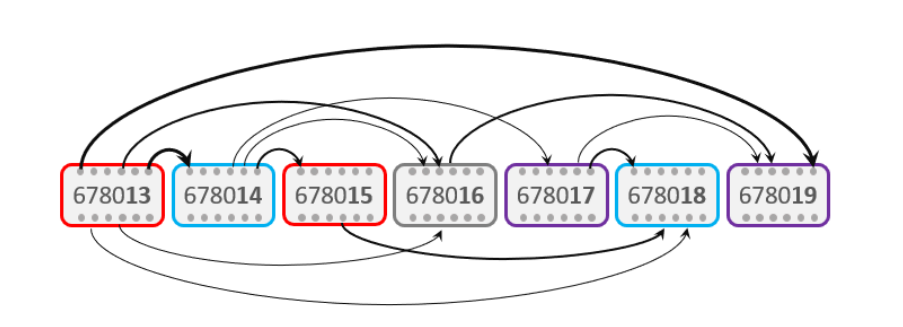
\includegraphics[keepaspectratio=true,scale=0.5]{Images/exampleBitvasVis.png}
    \caption{Visualizzazione generica BITVAS}
\end{figure}

In figura 3 è mostrato un esempio di visualizzazione adottata da BITVAS, il cui fulcro è una catena di blocchi.
Ognuno di essi è rappresentato da un rettangolo identificato da un numero che rappresenta la sua altezza nella blockchain, il cui colore del contorno sta ad indicare il miner o il mining pool che lo ha minato.
Nel caso in cui l'output di almeno una transazione all'interno di un blocco venga utilizzato come input in una transazione di un altro blocco, la relazione tra i due viene definita tramite una freccia, il cui spessore è definito dal numero di transazioni coinvolte.

Di fondamentale importanza è l'introduzione dei \emph{Cluster block}, ovvero un insieme di blocchi che vengono aggregati utili a determinate visualizzazioni, in quanto permette di rappresentare dei blocchi consecutivi dei quali non si è interessati ai dettagli.



\begin{figure}[H]
    \centering 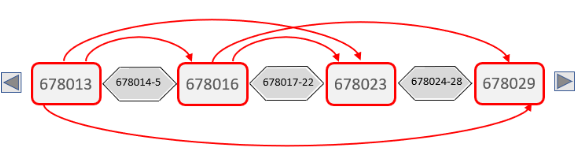
\includegraphics[keepaspectratio=true,scale=0.7]{Images/MinerVisualization2.png}
    \caption{Miner Visualization di  BITVAS}
\end{figure}

In figura 4 la visualizzazione presa in esame riguarda tutti i blocchi di un determinato arco temporale, che sono stati minati dallo stesso miner.
In questo caso i Cluster Blocks vengono utilizzati per trascurare i dettagli e le relazioni dei blocchi che non soddisfano i requisiti sopra citati. 


\subsection{Cenni al graph database di riferimento}
La crescente attenzione degli ultimi anni per le cryptovalute ha portato come conseguenza ad un aumento massiccio dei dati conservati nelle blockchain, la cui dimensione al giorno d'oggi, per quanto riguarda Bitcoin è di circa 590 Gigabyte \cite{blockchair}.
In genere, i tool di visualizzazione che prendono di mira tale mole di dati, non la utilizzano tutta, bensì applicano un filtraggio per ottenere solo quelli necessari all'adempimento delle richieste degli utenti.

Inoltre, le sole informazioni presenti nelle blockchain sono quelle riguardanti i blocchi, le transazioni e le relazioni tra essi, rappresentative dei flussi di Bitcoin, le quali possono essere limitate e in certi casi limitanti per analisi più approfondite.
Lo sviluppo del database a grafo è incentrato sulla possibilità di introdurre altri livelli di dettaglio, in grado di permettere una visione d'insieme di alcuni flussi di cryptovaluta.

L'obiettivo del database a grafo sviluppato è quello di aumentare la granularità delle informazioni presenti nella blockchain, aggregando queste ultime in cluster (ore, giorni, mesi e anni) collegati tra loro in base alle relazioni presenti ai livelli sottostanti.
In questo modo si possono reperire i flussi appartenenti ad un insieme di blocchi.
Questo approccio non solo migliora la comprensione dei flussi di cryptovaluta, ma riduce anche il carico computazionale necessario per l’estrazione delle informazioni, rendendo il processo di analisi più veloce e meno oneroso.

Inoltre, l’uso di un database a grafo permette di identificare pattern e anomalie nei flussi di criptovaluta che potrebbero non essere evidenti con un’analisi tradizionale. Ad esempio, è possibile tracciare il movimento di grandi quantità di Bitcoin tra diversi indirizzi, identificando potenziali attività sospette o comportamenti di mercato significativi. Questo livello di analisi avanzata è fondamentale per migliorare la sicurezza e la trasparenza delle transazioni in criptovaluta.

\thispagestyle{mystyle}




